\documentclass{scrartcl}
\usepackage{graphicx}
\usepackage{amsmath}
\usepackage{listings}
\usepackage{mathtools}
\usepackage{physics}
\usepackage{siunitx}
\usepackage{tikz}
\usepackage{mathtools}
\usepackage{rotating}
\usepackage{hyperref}
\usepackage{fancyhdr}

\pagestyle{fancy}
\fancyhf{}
\rhead{Jamie Grieser}
\lhead{Simulation Methods}
\rfoot{Page \thepage}

\definecolor{mygreen}{rgb}{0,0.6,0}
\definecolor{mygray}{rgb}{0.5,0.5,0.5}
\definecolor{mymauve}{rgb}{0.58,0,0.82}

\lstset{ 
	backgroundcolor=\color{white},   % choose the background color; you must add \usepackage{color} or \usepackage{xcolor}; should come as last argument
	basicstyle=\footnotesize,        % the size of the fonts that are used for the code
	breakatwhitespace=false,         % sets if automatic breaks should only happen at whitespace
	breaklines=true,                 % sets automatic line breaking
	captionpos=b,                    % sets the caption-position to bottom
	commentstyle=\color{mygreen},    % comment style
	deletekeywords={...},            % if you want to delete keywords from the given language
	escapeinside={\%*}{*)},          % if you want to add LaTeX within your code
	extendedchars=true,              % lets you use non-ASCII characters; for 8-bits encodings only, does not work with UTF-8
	frame=single,	                   % adds a frame around the code
	keepspaces=false,                 % keeps spaces in text, useful for keeping indentation of code (possibly needs columns=flexible)
	keywordstyle=\color{blue},       % keyword style
	language=Octave,                 % the language of the code
	morekeywords={*,...},            % if you want to add more keywords to the set
	numbers=left,                    % where to put the line-numbers; possible values are (none, left, right)
	numbersep=5pt,                   % how far the line-numbers are from the code
	numberstyle=\tiny\color{mygray}, % the style that is used for the line-numbers
	rulecolor=\color{black},         % if not set, the frame-color may be changed on line-breaks within not-black text (e.g. comments (green here))
	%showspaces=false,                % show spaces everywhere adding particular underscores; it overrides 'showstringspaces'
	showstringspaces=false,          % underline spaces within strings only
	showtabs=false,                  % show tabs within strings adding particular underscores
	stepnumber=2,                    % the step between two line-numbers. If it's 1, each line will be numbered
	stringstyle=\color{mymauve},     % string literal style
	tabsize=2,	                   % sets default tabsize to 2 spaces
	%title=\lstname                   % show the filename of files included with \lstinputlisting; also try caption instead of title
}

\begin{document}

\section*{Problem Sheet 4 - Exercise 1}
\subsubsection*{Part (b)}
The solutions of this exercise are based on the predefined template that was provided on the website. In the following, you can find the modifications that I performed to obtain the results shown below.
\begin{lstlisting}[title=Code for the computation of the center of mass and mass in the tree algorithm., language=Python, frame=single]
	for iz in range(0,2):
		for iy in range(0,2):
			for ix in range(0,2):
				id = self.nodelist[nodeid].childrenids[ix,iy,iz]
				cm, m = self.computemultipoles(id)
				if m != 0: # Ignore cells with mass 0 as they do not contribute
					mass = mass + m
					for i in range(0,3):
						cenm[i] = (m * cm[i] + (mass - m) * cenm[i])/mass
\end{lstlisting}

\begin{lstlisting}[title=Code for the computation of the partial force on the particle.,language=Python, frame=single]
if angle < anglemax or self.nodelist[nodeid].leaf == 1:
	#
	# This is a small enough branch or it is a leaf.
	# In either case just use the node's cm and mass.
	# But avoid self-attraction!
	# Particle mass is 1.0
	distance = (self.nodelist[nodeid].cm[0] - self.particles[pid][0])**2 \
						+ (self.nodelist[nodeid].cm[1] - self.particles[pid][1])**2 \
						+ (self.nodelist[nodeid].cm[2] - self.particles[pid][2])**2
	# avoiding self-attraction
	if distance != 0:
		for i in range(0, 3):
			force[i] = self.nodelist[nodeid].mass * \
			np.power(distance + 0.001**2, -3/2) \
			* (self.particles[pid][i] - self.nodelist[nodeid].cm[i])
\end{lstlisting}

\begin{lstlisting}[title=Code for the computation of the exact forces on a particle.,language=Python, frame=single]
def exact_force(self, pid):
	force = [0., 0., 0.]
	for id in range(0, len(self.particles)):
	# avoid self-interaction:
	if id != pid:
		dist = np.power((self.particles[pid][0] - self.particles[id][0]) ** 2
				+ (self.particles[pid][1] - self.particles[id][1]) ** 2
				+ (self.particles[pid][2] - self.particles[id][2]) ** 2
				+ 0.001 ** 2, -3/2)
		for j in range(0, 3):
			force[j] = force[j] + dist * (self.particles[pid][j] - self.particles[id][j])
	return force
\end{lstlisting}

\begin{lstlisting}[title=Code for the computation of the exact forces on a particle.,language=Python, frame=single]
def all_exact_forces(self):
	nrp = len(self.particles)
	for pid in range(nrp):
		self.forces[pid][:] = self.exact_force(pid)
\end{lstlisting}
\subsubsection*{Part (c)}

The following piece shows how the average arithmetic error \( \langle \eta \rangle \) is calculated.
\begin{lstlisting}[title=Code for the computation of the relative average error.,language=Python, frame=single]
def distance(particle1, particle2):
	squared_dist = (particle1[0] - particle2[0]) ** 2 \
					+ (particle1[1] - particle2[1]) ** 2 \
					+ (particle1[2] - particle2[2]) ** 2
	return np.sqrt(squared_dist)


for i in range(0, len(particles)):
	avgerror = avgerror + distance(fapprox[i], fexact[i]) \
				/ distance(fexact[i], [0., 0., 0.])

avgerror = avgerror / nparticles
print("The average error was computed to be:", avgerror)
\end{lstlisting}

The algorithm to count the number of node-particle interactions per particle was written in a way that it only counts interactions with nodes with non-zero mass. See the attached code for further information (look at the function gforce).

\subsubsection*{Part (d)}

The following tables show the computation time, average arithmetic error and average nodes per particle for several numbers of particles and different opening angles.
\begin{table}[ht]
	\centering
	\begin{tabular}{|l|l|l|l||l|}
		\hline
		Time [s] & 0.2 & 0.4 & 0.8 & Brute Force \\ \hline
		5000        & 298.61       	   & 79.62     	   	& 17.30  & 131.78 \\ \hline
		10000       & 773.83           & 187.43			& 38.39  & 526.40  \\ \hline
		20000       & 1941.86          & 434.21        	& 84.68  & 2097.46\\ \hline
		40000       & 4789.59          & 1001.59       	& 187.85 & 8297.63 \\ \hline
	\end{tabular}
	\caption{Calculation time for different number of particles and opening angles in comparison to the brute force algorithm. One can easily see the logarithmic scaling for the tree algorithm and the quadratic scaling in the brute-force case.}
\end{table}

\begin{table}[ht]
	\centering
	\begin{tabular}{|l|l|l|l|}
		\hline
		Interactions [1] & 0.2 & 0.4 & 0.8 \\ \hline
		5000        & 1886.8       	   & 578.3     	   & 133.6  \\ \hline
		10000       & 2603.9           & 705.5         & 152.7  \\ \hline
		20000       & 3480.8	       & 849.4         & 173.73 \\ \hline
		40000       & 4433.9           & 997.220225    & 194.6  \\ \hline
	\end{tabular}
	\caption{Average Number of interactions for different number of particles and opening angles.}
\end{table}

\begin{table}[ht]
	\centering
	\begin{tabular}{|l|l|l|l|}
		\hline
		\( \eta \) [1] & 0.2 & 0.4 & 0.8 \\ \hline
		5000        & 0.0003           & 0.0029        & 0.0154   \\ \hline
		10000       & 0.0003           & 0.0025        & 0.0131   \\ \hline
		20000       & 0.0003           & 0.0022        & 0.0112   \\ \hline
		40000       & 0.0003           & 0.0022        & 0.0100   \\ \hline
	\end{tabular}
	\caption{Average relative error per particle for different number of particles and opening angles in comparison to the brute force algorithm.}
\end{table}
\newpage
\subsubsection*{Part (e)}
The plot of the data points and fit function is displayed in \href{fig:calctime}{Figure 1}. I decided to fit a function of the type \( y = a \cdot x^b \) to the given function  with the parameters \( a = 0.0027\) and \( b = 1.209 \). From this, the estimated computation time for \( 10^{10} \) particles is approximately \( 105.3\text{ Years} \).
\begin{sidewaysfigure}
	\centering
	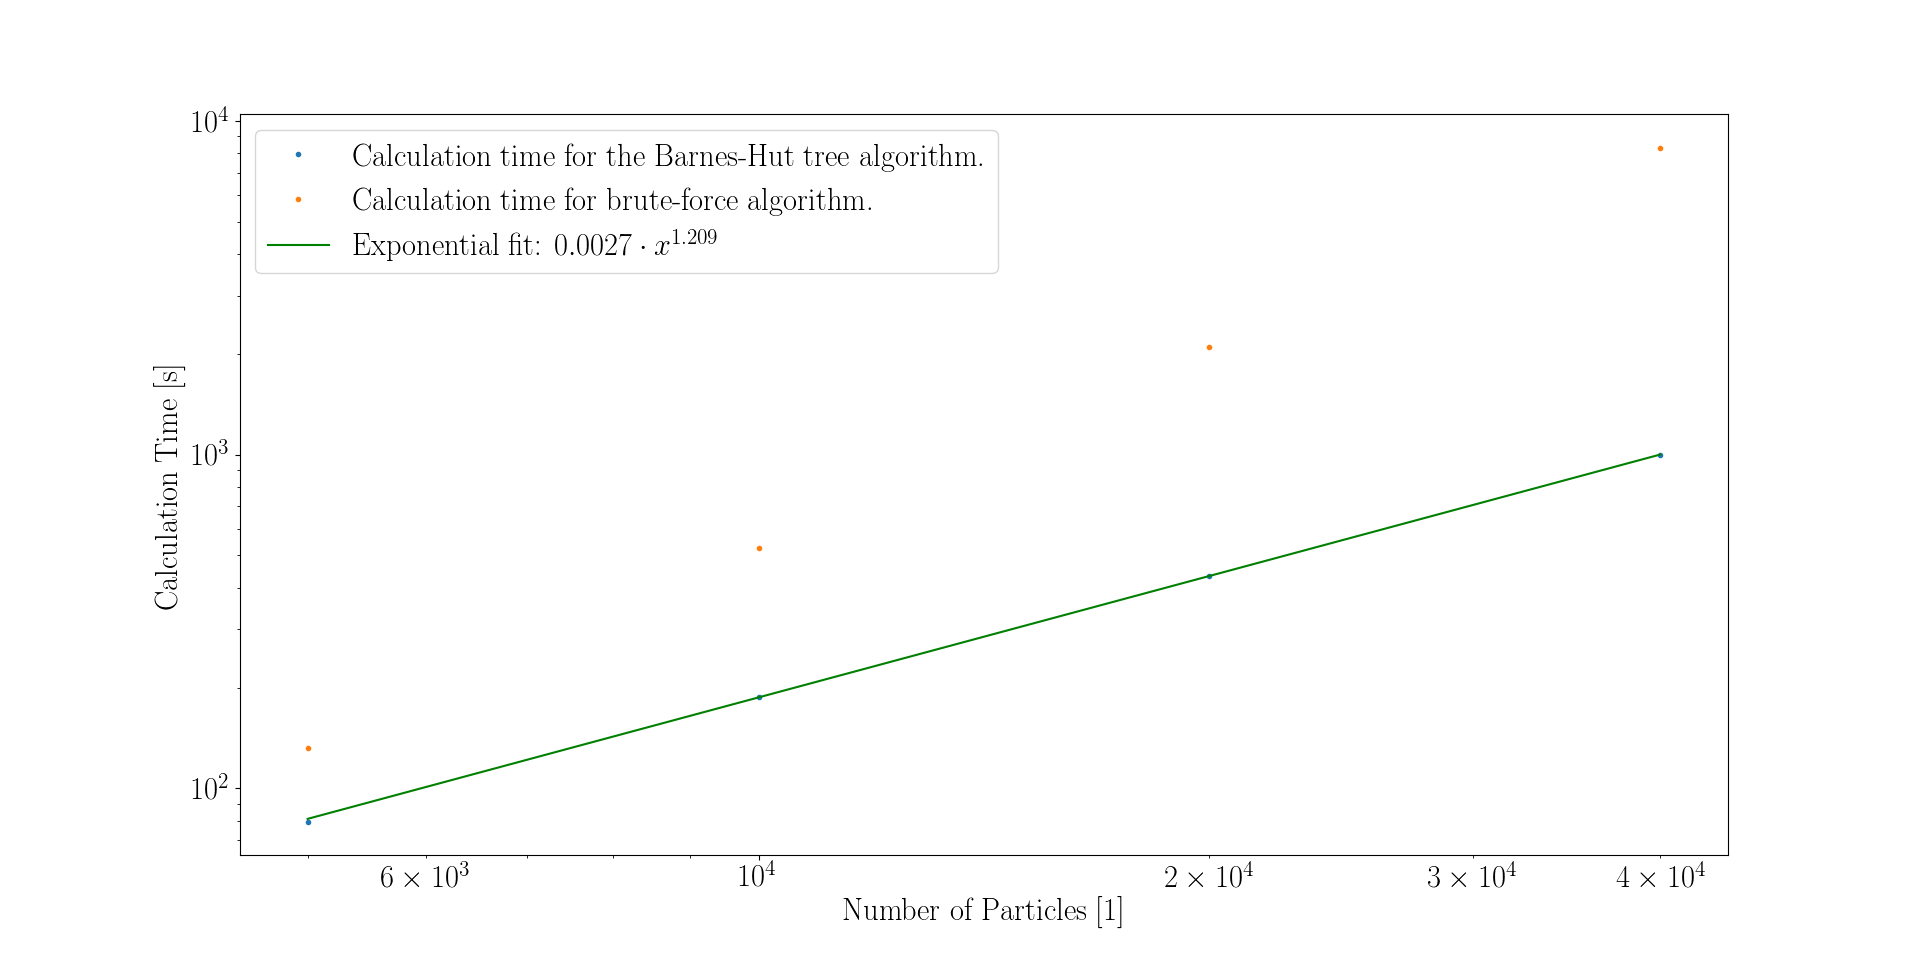
\includegraphics[width=1.0\linewidth]{CalcTime}
	\caption{Plot of the calculation time for the brute force and the tree algorithm with opening angle \( \theta = 0.8\)}
	\label{fig:calctime}
\end{sidewaysfigure}


\end{document}
